\section{Two-way calls}
\label{sec:two-way}

Two-way calls (or ``two-leg calls'') are the normal telephone calls between to participants of the AskoziaPBX.
User A calls another user (perhaps User B who has to be registered), makes a phone call and hangs up.

In \texttt{sip} diagram, the scenario looks as follows:
\begin{figure} [!ht]
\centering
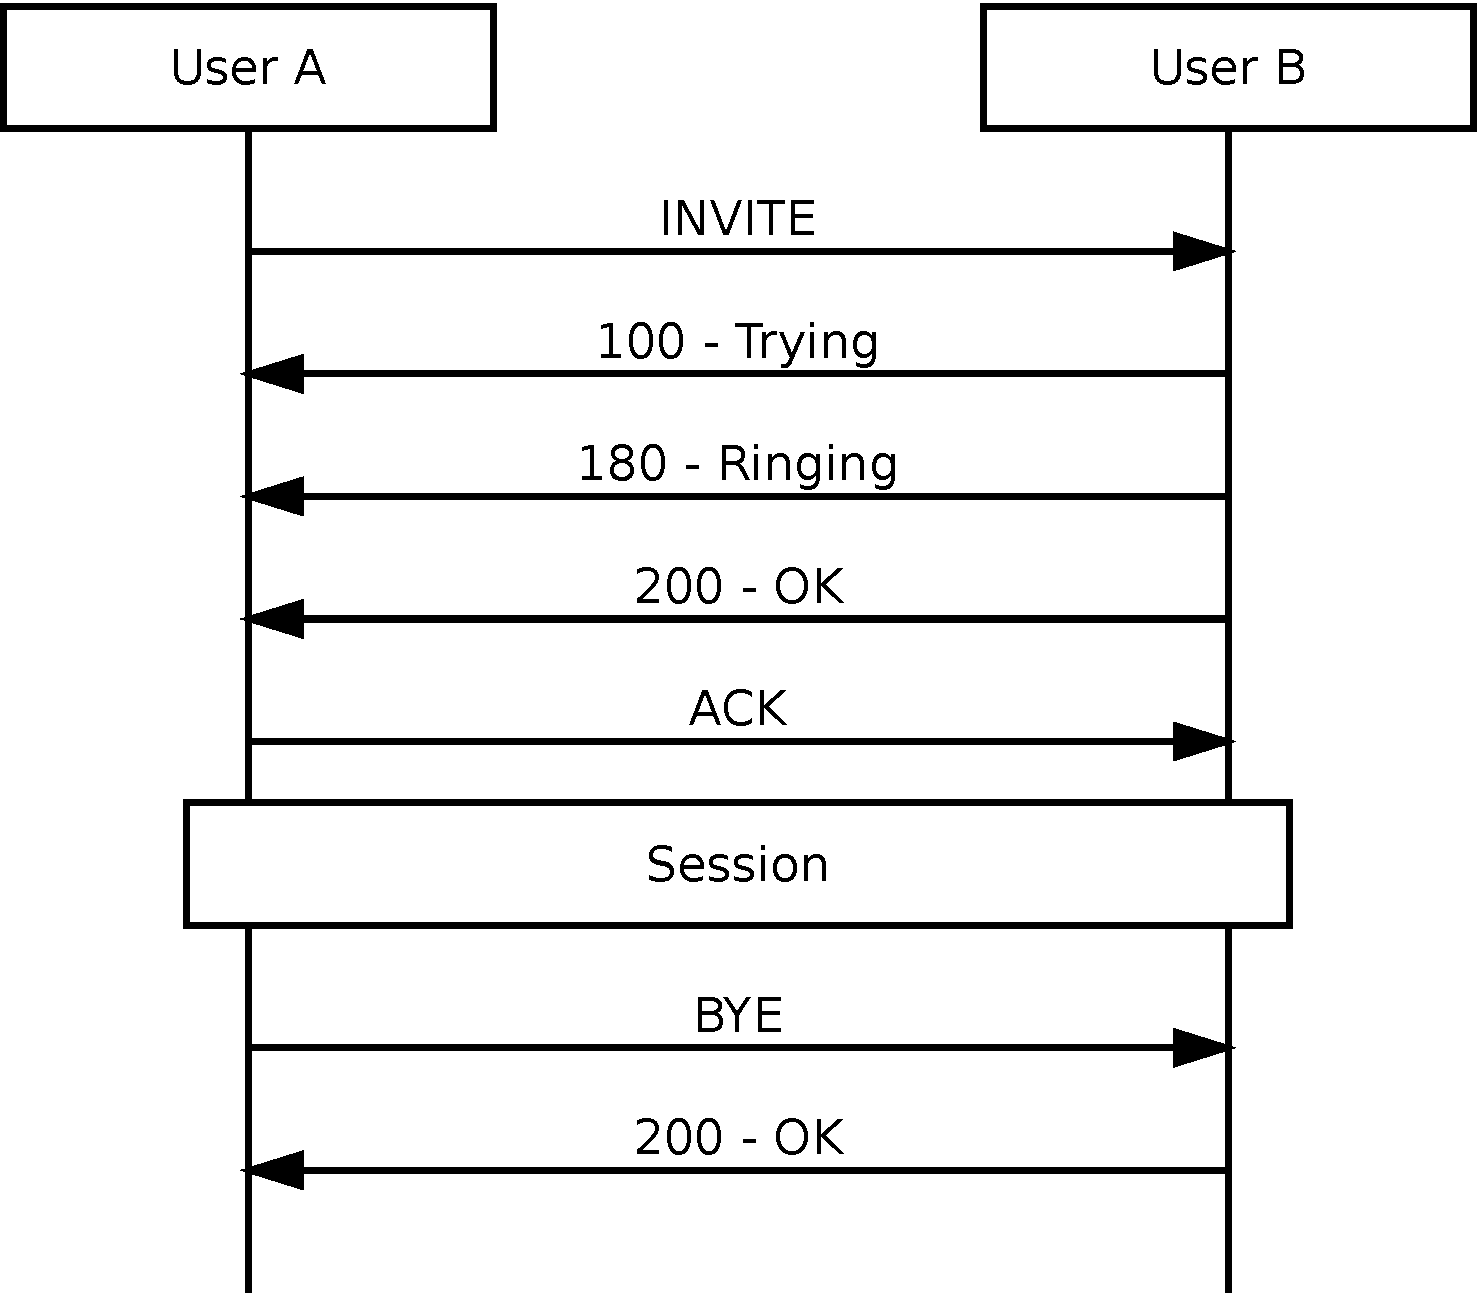
\includegraphics [width=10cm] {twoway-1}
\caption{SIP diagram of a two-way call}
\end{figure}

This scenario is implemented like that, the original xml scenarios are deposed in the appendix:
\begin{figure} [!ht]
\centering
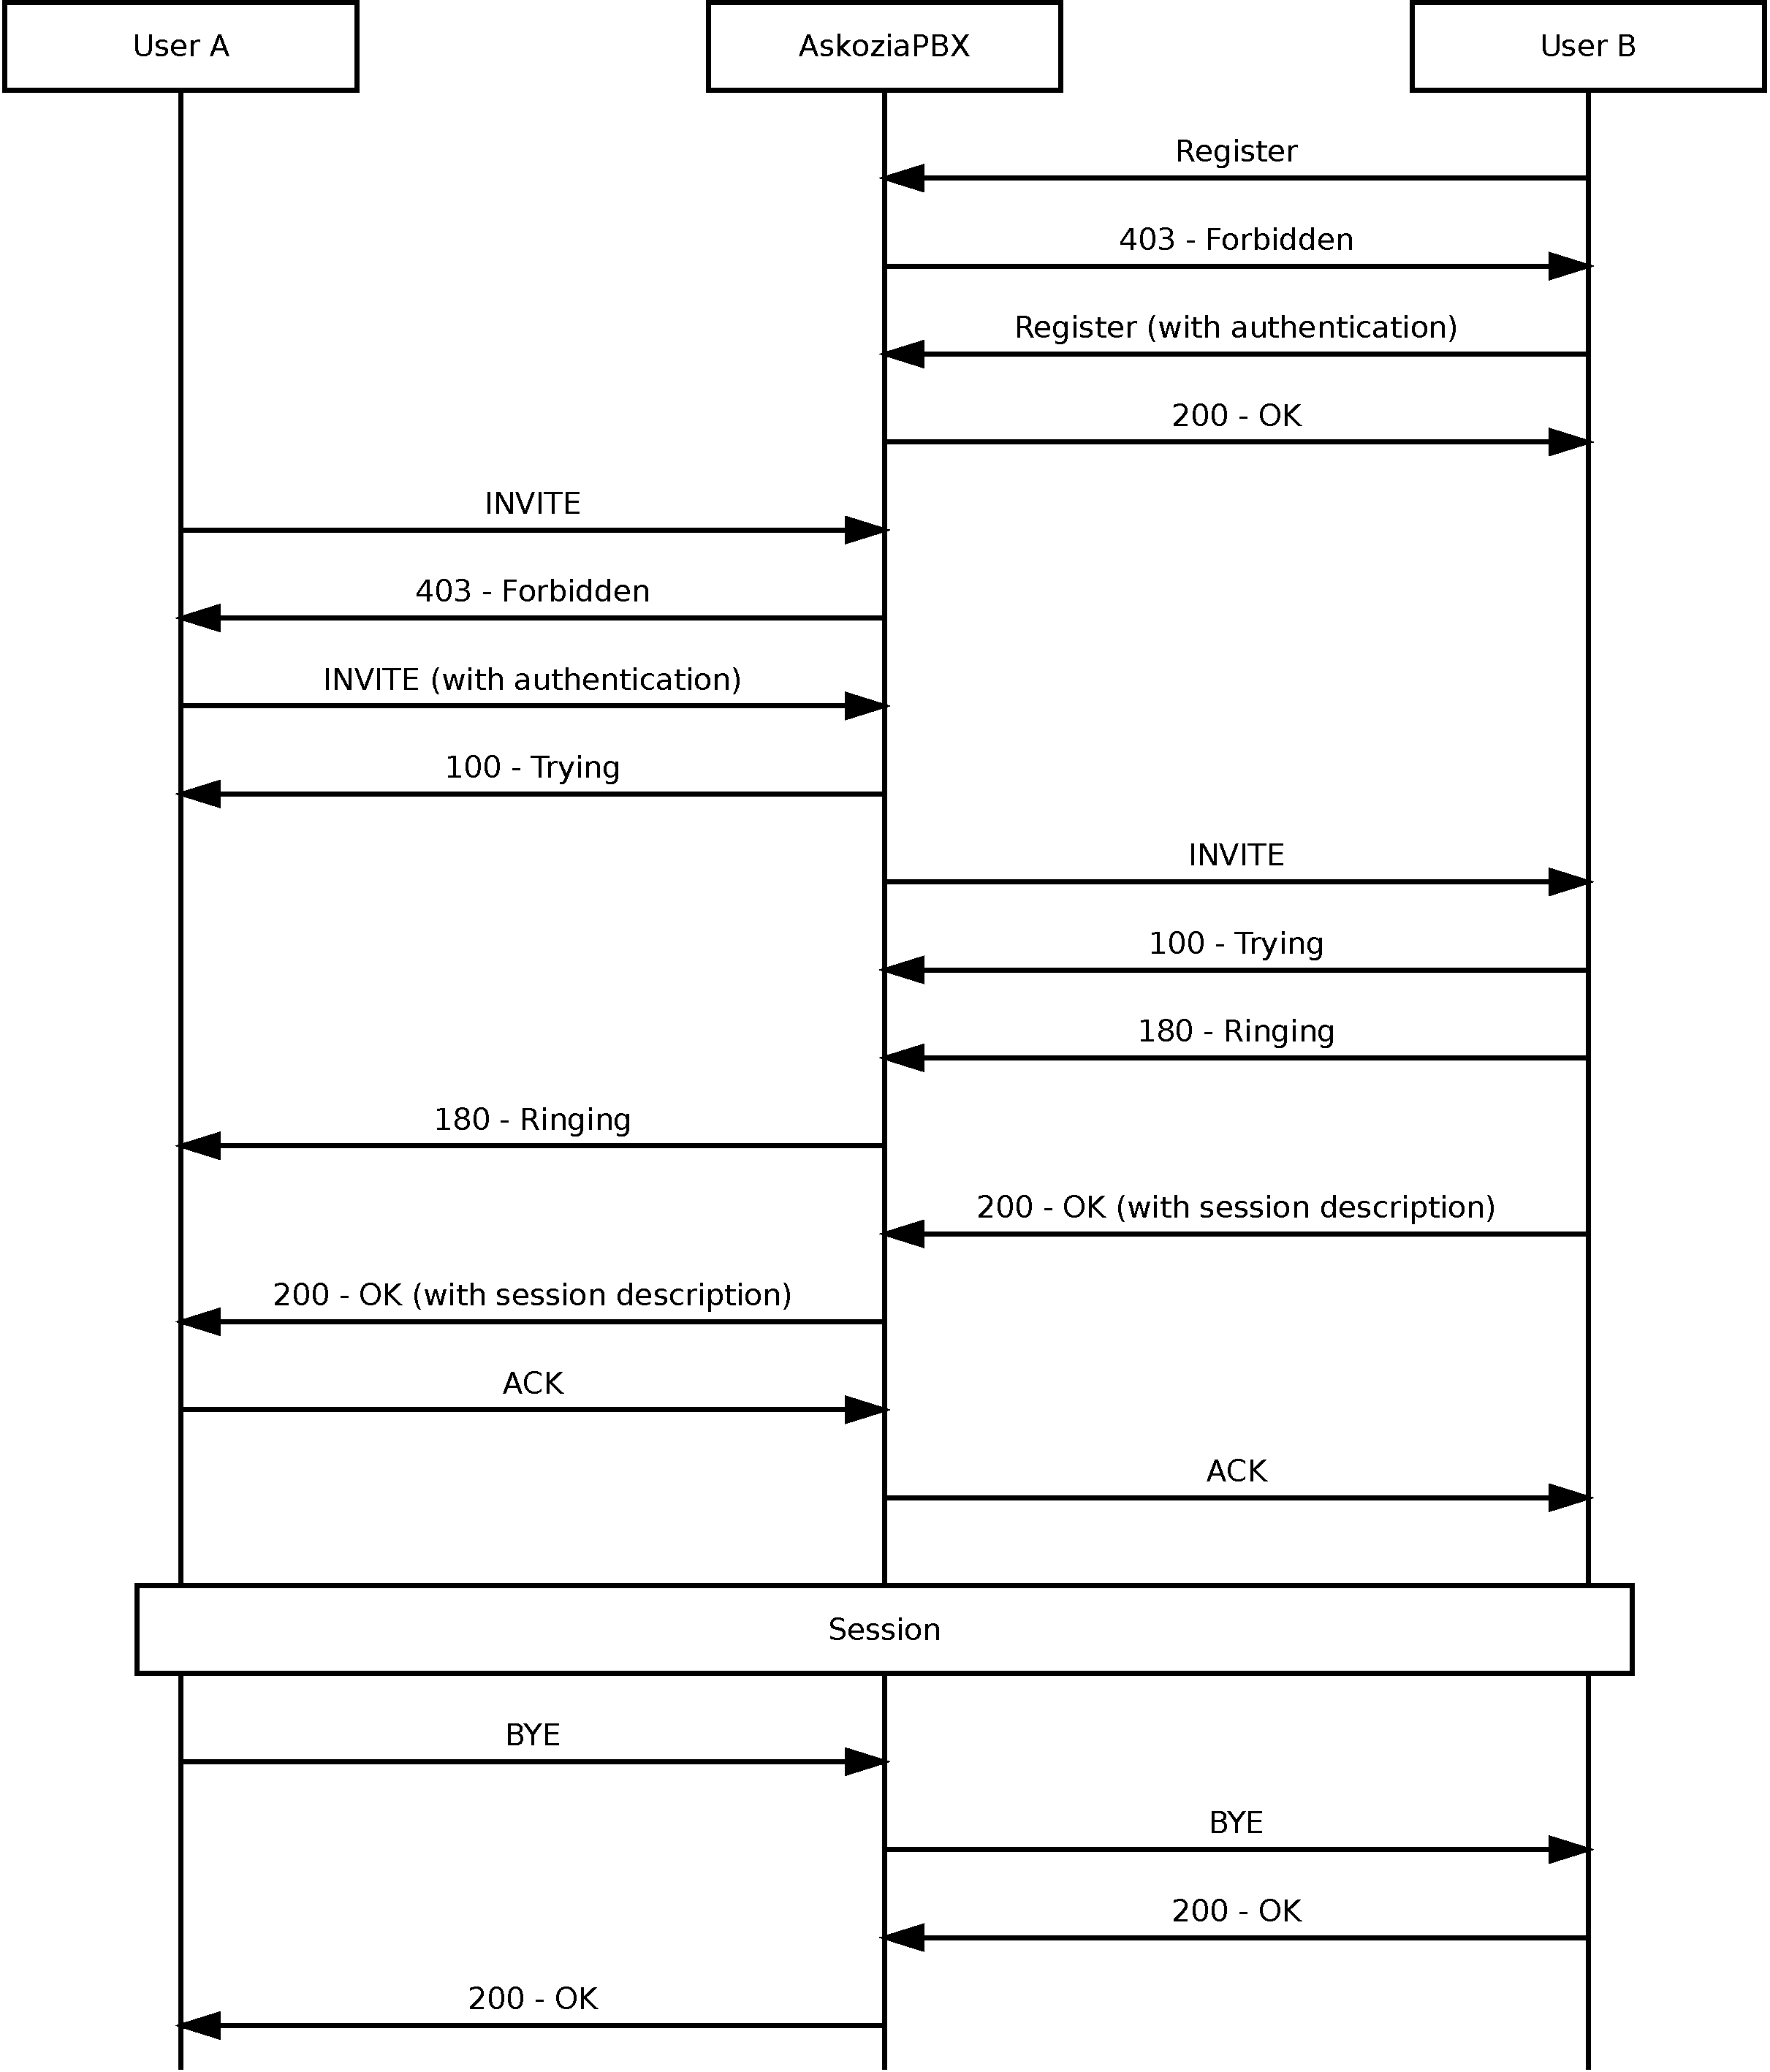
\includegraphics [width=15cm] {twoway-2}
\caption{Scenario of a two-way call}
\end{figure}

The next diagramm shows the process of a complete two-way test: \newpage
\begin{figure} [!ht]
\centering
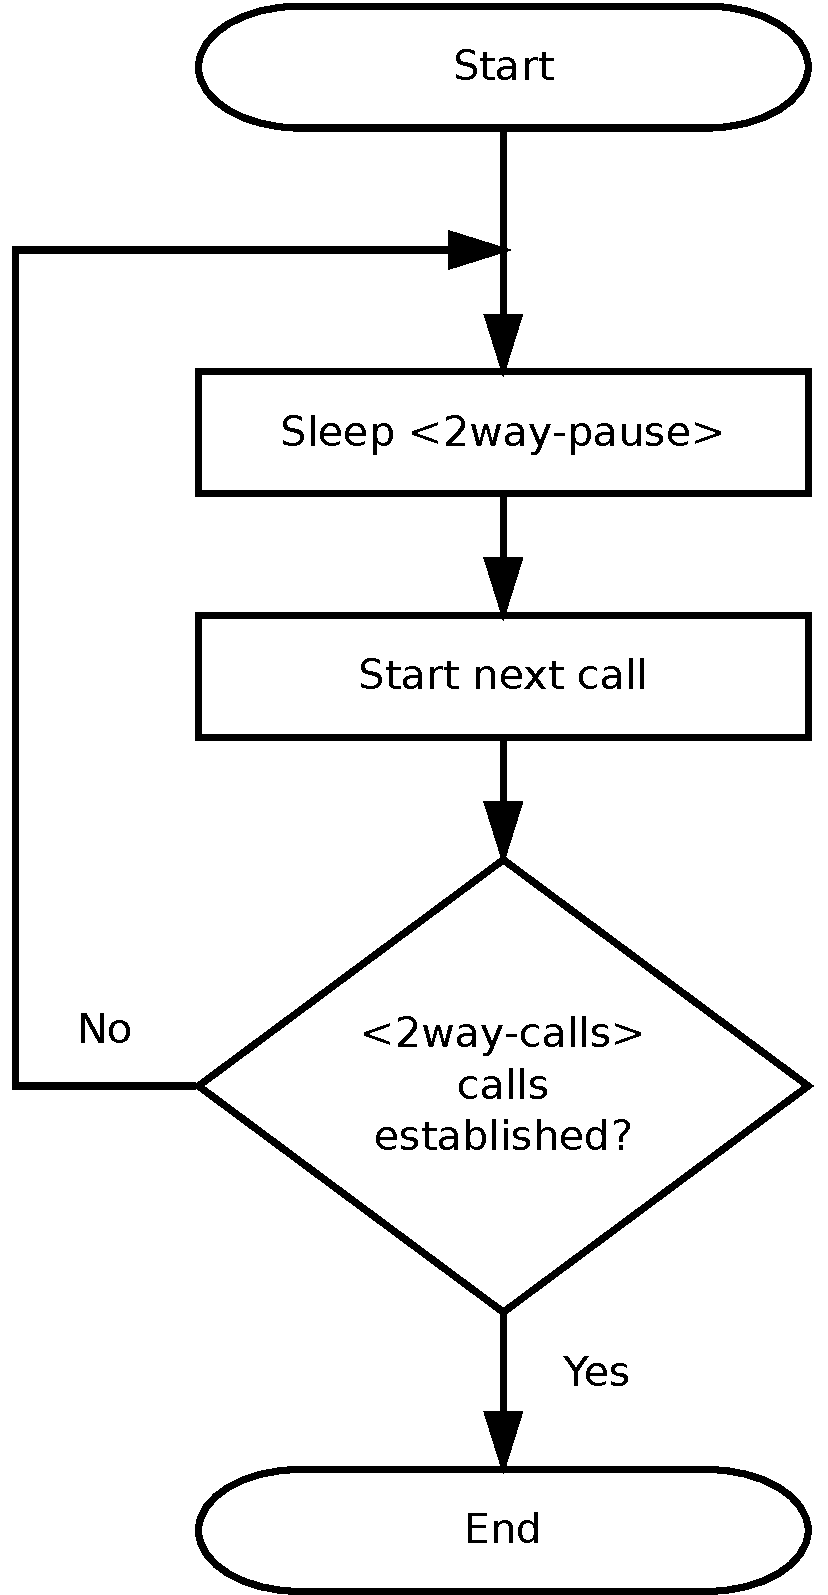
\includegraphics [width=6cm] {twoway-3}
\caption{Complete two-way test}
\end{figure}

The number of calls is increased step-by-step. After every call, the script waits for the with
the script call passed parameters time to record the CPU load values. For executing two-way calls, there
are the following commands used:
\begin{lstlisting}[breaklines=true,label=code:twoway-invite,caption={sipp command for inviting User B} ]
my $constant = "'$sipp' -aa -inf '$users_twoway_file' -m $current_call -i $local_ip ";
my $reg_cmd = $constant . "-p $sip_dst_port -mp $rtp_dst_port -sf '$reg_scen' $ask_ip 2>&1";
my $acc_cmd = $constant . "-p $sip_dst_port -mp $rtp_dst_port -sf '$acc_scen' -bg $ask_ip 2>&1 &";
my $inv_cmd = $constant . "-p $sip_src_port -mp $rtp_src_port -sf '$inv_scen' $ask_ip 2>&1";
my $der_cmd = $constant . "-p $sip_dst_port -mp $rtp_dst_port -sf '$der_scen' $ask_ip 2>&1";
\end{lstlisting}

\texttt{\$constant} is used because some settings of the current sipp call are needed in all other calls (register, accept, invite and deregister), too.
So, it is not neccessary (and more comfortable) to write them down once and not four times. You can inform yourself about the used parameters by
reading the sipp manpage (the appendix contains the sipp manpage).
